
\begin{figure*}[t]
\vspace{-2em}
\centering
\begin{subfigure}[b]{0.5\textwidth}
  \centering
  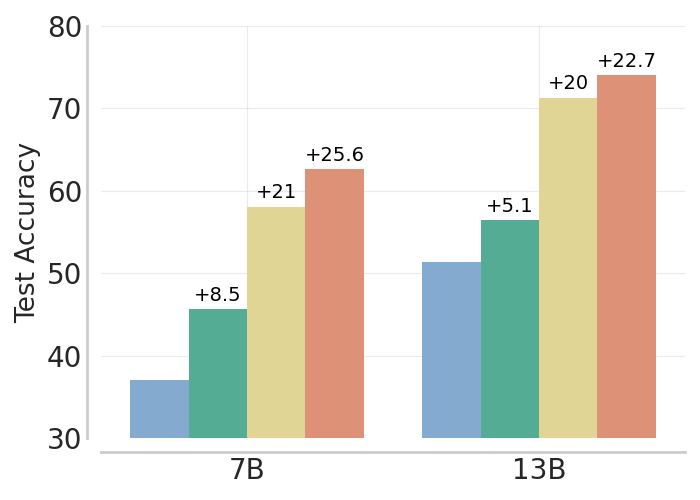
\includegraphics[scale=0.39]{icml2023/figs/abs_with_rel/gsm8k_abs_with_rel.png}
  \caption{GSM8K for 7B and 13B sizes}
    \label{fig:gsm8k}
\end{subfigure}%
\begin{subfigure}[b]{0.5\textwidth}
  \centering
  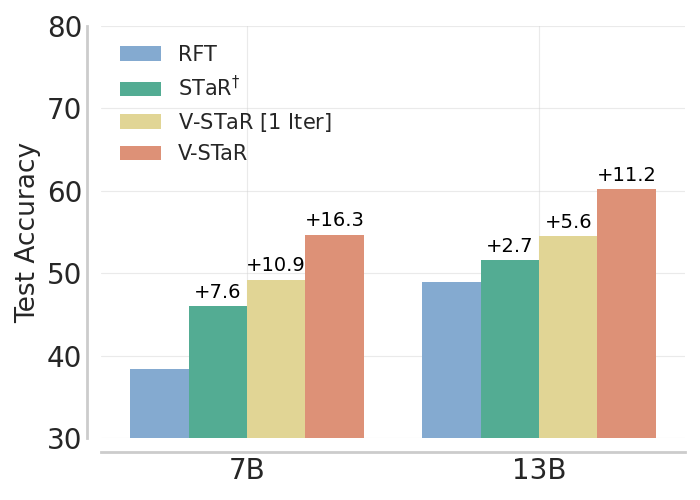
\includegraphics[scale=0.39]{icml2023/figs/abs_with_rel/mbpp_abs_with_rel.png}
  \caption{MBPP for 7B and 13B sizes}
    \label{fig:mbpp}
\end{subfigure}%
\caption{\textbf{Pass$@1$ and Best-of-64 scores for generator-only and verifier-based methods}. Numbers above each bar represent the absolute improvement over RFT. \vstar{}[1 Iter] baseline is trained with data consisting of $3\times16$ completions per query for one iteration only. \stardag and \vstar{} are trained using iterative data collection (i.e. 16 completions generated per query at each iteration). At test time, \revision{Best-of-64 is calculated using \autoref{eq:ver_at_k} on 128 candidate answers sampled per problem from the generators}. \vstar{} 7B performs on par with CodeLLaMA 34B, which has a zero-shot Pass$@1$ of 55\% on MBPP. }
\label{fig:results_rft_1iter}
\vskip -0.03in
\end{figure*}


% \vskip -0.2in
% \vspace{-0.1}
\section{Empirical results}

\label{sec:exp_desc}
To demonstrate the effectiveness of \vstar{}, we conduct experiments on two widely used datasets:
GSM8K~\citep{DBLP:journals/corr/abs-2110-14168} for solving math problems, and MBPP~\citep{austin2021program} for code-generation problems. We also evaluate the transfer generalization performance of \vstar{} using Hendrycks' MATH~\citep{DBLP:conf/nips/HendrycksBKABTS21} and HumanEval~\citep{chen2021codex}. Specifically, for math reasoning, we only train our generators and verifiers using GSM8K training data and evaluate them on the whole GSM8K test set and a subset of MATH test set\footnote{This subset includes a total 150 problems of Level 1 difficulty in MATH with question types of \textit{algebra}, \textit{Counting \& probability}, \textit{prealgebra} and \textit{number theory} where the final answer is a number and no latex exists in the question.}.
For code generation, we train our models using the MBPP training data and evaluate them on the full test sets of MBPP and HumanEval.
% formatted using the MBPP prompt template.


% \subsection{Models}
\paragraph{Models} For experiments, we fine-tune LLaMA2 \citep{DBLP:journals/corr/abs-2307-09288} and CodeLLaMA \citep{DBLP:journals/corr/abs-2308-12950} 7B and 13B models using LoRA \citep{DBLP:conf/iclr/HuSWALWWC22}. 
Generators are trained with a causal language modeling objective, and our baseline (\vstar [1 Iter]) and \vstar{} verifiers are trained using DPO. The reference policy $G_{\text{SFT}}$ for DPO is trained on the original training data for 2 and 3 epochs for GSM8K and MBPP, respectively. See \autoref{sec:dpo_verifier} for details. 
%% RA.1.26: Ablation to use DPO reward -- the likelihood ratio should be compared for this design choice (maybe in appendix or main dpeending on space)

% \vspace{-0.2cm}
\paragraph{Data generation} For each iteration, $k=16$ completions are sampled per query from the previous iteration's generator.
% The data for each iteration is generated by sampling from the previous iteration's generator. 
For GSM8K, the first iteration samples are from a generator trained solely on the original GSM8K training data for 2 epochs. For MBPP, this data is from a \revision{3-shot pretrained CodeLLaMA} (see \autoref{app:mbpp_shots}).
Completions are labeled for correctness by checking the final answer for math problems and running test cases for coding problems.% \vspace{-1}


\begin{figure*}[t]
\vskip -0.1in
\centering
\begin{subfigure}[b]{0.5\textwidth}
  \centering
  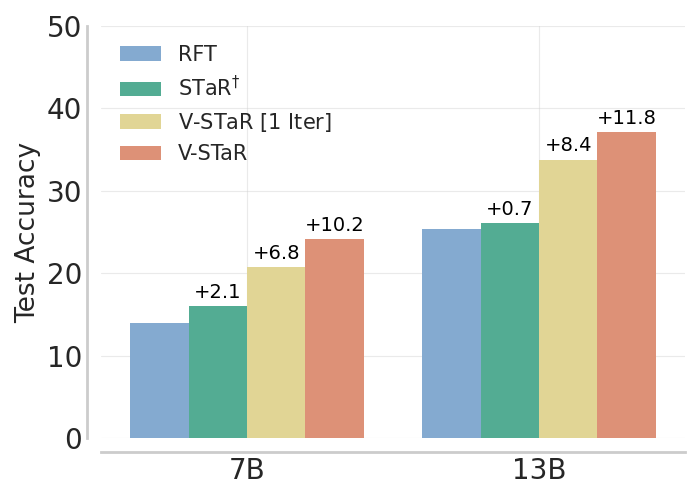
\includegraphics[scale=0.39]{icml2023/figs/abs_with_rel/MATH_abs_with_rel.png}
  \caption{GSM8K $\rightarrow$ MATH Subset}
    \label{fig:math}
\end{subfigure}%
\begin{subfigure}[b]{0.5\textwidth}
  \centering
  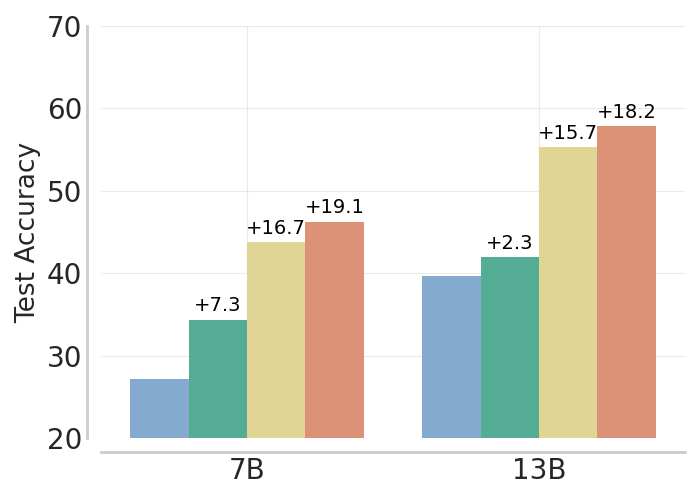
\includegraphics[scale=0.39]{icml2023/figs/abs_with_rel/humaneval_abs_with_rel.png}
  \caption{MBPP $\rightarrow$ HumanEval}
    \label{fig:humaneval}
\end{subfigure}%
\caption{\textbf{Out-of-domain transfer evaluation}: Pass$@1$ and Best-of-$64$ for generators and verifiers with absolute improvement over RFT shown above each bar. Models trained on GSM8K are evaluated on a subset of MATH test set (\autoref{sec:exp_desc}), and models trained on MBPP are evaluate on HumanEval test set. \vstar{} 7B performs close to CodeLLaMA 34B which has a zero-shot Pass$@1$ of 48\% on HumanEval.}
\label{fig:transfer}
\vskip -0.22in
\end{figure*}



\subsection{Baselines and metrics}
\label{sec:baselines}

We run \vstar{} for 3 iterations and sample $k=16$ solutions at each iteration to augment $\mathcal{D}_{\text{GEN}}$ and $\mathcal{D}_{\text{VER}}$. To assess the gains from our iterative approach, we compare against a number of baselines (\autoref{tab:bootstrap_methods}):
\begin{enumerate}[label=\arabic*.,left=0pt,nosep]
\item \textbf{SFT}: Standard fine-tuning (\autoref{eq:sft}) on training data without any self-improvement or test-time verification.
\item \textbf{\stardag}: Bootstrapping a generator by sampling $k=16$ completions per query for 3 iterations, see \autoref{sec:si_approach}.
% A generator is bootstrapped by sampling K=16 completions per query for 3 iterations, see \autoref{sec:si_approach}. 

\item \textbf{RFT}: Running \stardag by sampling $3\times16$ completions for only 1 iteration, see \autoref{sec:si_approach}.

\item \textbf{Verification} (SFT + Verifier): Generating $3\times16$ completions using SFT generator to train a verifier, as described in~\autoref{sec:dpo_obj}. This is similar to ORM verification approach by \citep{DBLP:journals/corr/abs-2110-14168} but empirically performs better (\autoref{fig:ver_at_k}).

\item \textbf{\vstar~[1 Iter]}: Bootstrapping a generator and training a verifier for 1 iteration with $k = 3\times16$ completions from $G_{\text{SFT}}$, so that the total generation budget matches \vstar. This baseline also corresponds  to \textbf{RFT + Verifier}.

\item \textbf{Self-consistency / Majority Voting}~\citep{wang2023making}: An alternative to use test-time compute without verifiers: sample multiple solutions from \stardag generator and pick the majority-vote answer.

\end{enumerate}


At inference, we generate 128 candidate solutions for each test problem using the generator. We report Pass$@1$ accuracy for the generators, which estimates the probability that an answer randomly sampled from the generator is correct. Best-of-64 accuracy is used for all verifier-based methods, using the formula in (\autoref{eq:ver_at_k}), as well as the self-consistency baseline. %We also report majority voting~\citep{DBLP:conf/iclr/0002WSLCNCZ23} performance as a strong baseline, following \citet{DBLP:journals/corr/abs-2110-14168, DBLP:journals/corr/abs-2305-20050}. 
\begin{figure*}[t]
\vskip -0.2in
\centering
\begin{subfigure}[b]{0.5\textwidth}
  \centering
  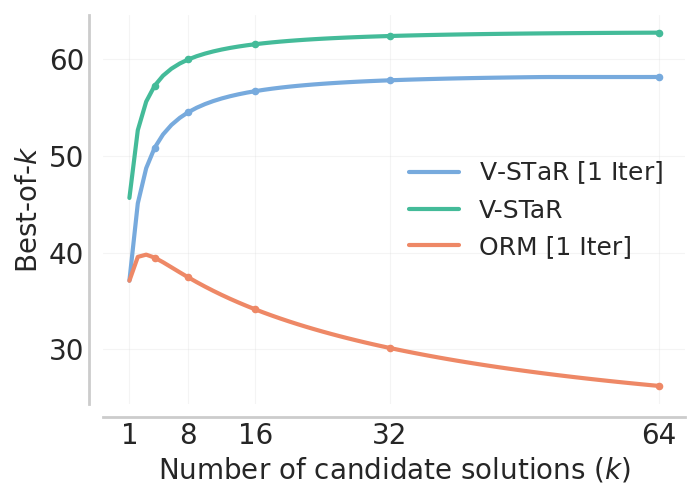
\includegraphics[scale=0.39]{icml2023/figs/ver_at_k/gsm8k_ver_at_k_colm.png}
  \caption{GSM8K Best-of-$k$}
    \label{fig:gsm8k_ver_at_k}
\end{subfigure}%
\begin{subfigure}[b]{0.5\textwidth}
  \centering
  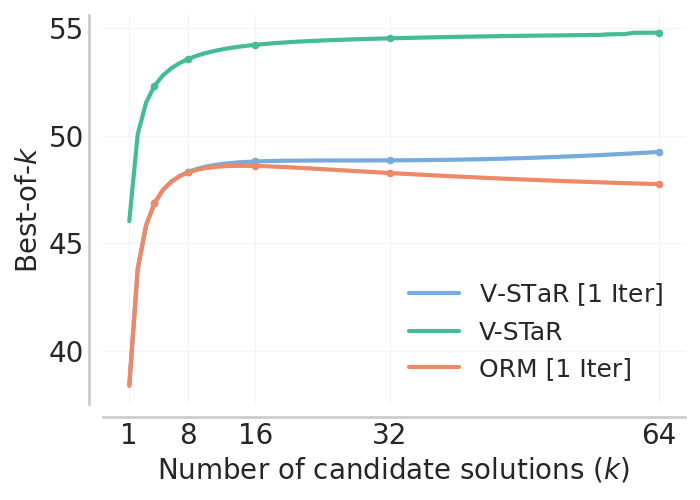
\includegraphics[scale=0.39]{icml2023/figs/ver_at_k/mbpp_ver_at_k_colm.png}
  \caption{MBPP Best-of-$k$}
    \label{fig:mbpp_ver_at_k}
\end{subfigure}%
\caption{\textbf{Best-of-k test accuracy} of \vstar{}, \vstar{}~[1 Iter], and outcome-supervised reward model (ORM) style verifier 7B models, measured by \autoref{eq:ver_at_k}. Best-of-$1$ is equivalent to not having a verifier and is equal to Pass$@1$ of the generator.}
\label{fig:ver_at_k}
\vskip -0.25in
\end{figure*}
\subsection{\revision{Reliable estimation of Best-of-$k$ accuracy}}

\label{sec:verifier_k}
% \vspace{-0.03in}
To estimate accuracy with test-time \revision{verifiers}, \revision{\cite{DBLP:journals/corr/abs-2110-14168, DBLP:journals/corr/abs-2305-20050} repeat the following procedure several times} and average the results: sample $k$ solutions, rank them using a verifier and take the top scoring one as the predicted answer. However, computing \revision{this best-of-$k$ accuracy can have high variance and is expensive}. Instead, \revision{to measure the best-of-$k$ accuracy reliably}, we propose two methods, akin to how Pass$@k$ is computed~\citep{chen2021codex}. 
To do so, we estimate the probability that out of $k$ samples drawn without replacement from a fixed set of $N$ (for $N > k$) samples, the one with the highest verifier score is correct. The best-of-$k$ is calculated by repeating this process $M$ times and taking the average. Assuming there are no duplicate verifier scores this can be done efficiently (see \autoref{app:ver_at_k_understand_pls} in appendix), using the following formula:
% \begin{wrapfigure}[4]{l}{0.45\textwidth}
\begin{equation}
    % \text{Verifier}@k := \frac{\sum_{i=0}^{N-k} \binom{N-i-1}{k-1}\alpha_i}  {\binom{N}{k}}
    \text{Best-of-}k := \frac{1}{\binom{N}{k}}\sum_{i=0}^{N-k} \binom{N-i-1}{k-1}\alpha_i
    \label{eq:ver_at_k}
\end{equation}
% \end{wrapfigure}
where $[\alpha_0, \dots, \alpha_{N-1}]$ are the binary correctness values (0 or 1) for the $N$ candidates $y_i$ sorted in decreasing order by their verifier score. The numerator here can be derived by considering subsets where the top-ranked candidate is $y_i$ for all possible values of $i \in \{0,\dots,N-k-1\}$.


% \vspace{-0.0259in}
\subsection{V-STaR on Math Reasoning and Code Generation}
As shown in \autoref{fig:results}, \vstar{} shows consistent gains across GSM8K, MBPP, MATH subset and HumanEval test sets for LLaMA2 7B and 13B models (\autoref{fig:results_13B}) over baselines.
In math, we report absolute improvement of 6 to 17\% in test accuracy over \stardag~and Verification, and 4 to 12\% in code generation tasks.
% The verifier in V-STaR~[1 Iter] is similarly trained on correct and incorrect solution pairs from $k=3\times16$ samples per problem. 
%V-STaR shows consistent gains on both tasks and model sizes. 
The gains over \vstar{}~[1 iter] in~\autoref{fig:results_rft_1iter} show that iteratively generating solutions to collect verifier training data results in a better distribution and quality compared to a non-iterative approach with the same generation budget. 
We show gains in each iteration of generator and verifier on MBPP in \autoref{fig:mbpp_heatmap}. 
We also trained a 4th iteration of generator and verifier on MBPP which led to a marginal gain of 0.3\%.

\looseness=-1
\textbf{Out-of-domain performance of V-STaR}. The generators and verifiers trained on MBPP are evaluated on HumanEval, while those trained on GSM8K are evaluated on a subset of MATH test set (see~\autoref{fig:results} and~\autoref{fig:transfer}). 
In general, we observe lower absolute Pass$@1$ and Best-of-$64$ scores for all methods as these two tasks are considered to be more difficult than GSM8K and MBPP. That said,
Iterative \vstar{} outperforms baselines, and \vstar{}~[1 iter] on both tasks and across model sizes. 
Utilizing incorrect solutions to train verifiers results in large improvements than just bootstrapping with correct model generated solutions using \stardag or RFT.
% We do not see a pattern of larger gain from V-STaR in one model size over the other across tasks. 
\begin{figure*}[t]
\vskip -0.2in
\centering
\begin{subfigure}[b]{0.5\textwidth}
  \centering
  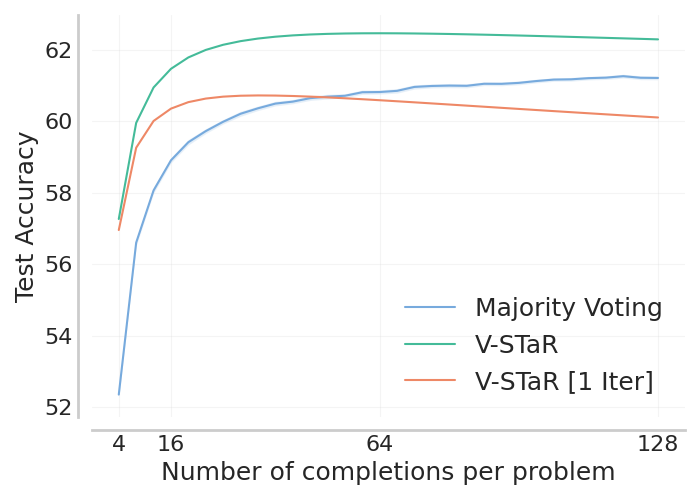
\includegraphics[scale=0.39]{icml2023/figs/maj_vs_ver_colm.png}
  % \caption{Test accuracy of 7B V-STaR compared to \vstar{}[1 Iter] and majority voting~\citep{DBLP:conf/iclr/0002WSLCNCZ23} across different numbers of candidate solutions generated on GSM8K. We subsample candidate solutions from $N=1000$ generations. V-STaR can rank over a reasonably large number of candidate solutions. We compute 95\% confidence interval for majority voting using 256 trials.}
    
\end{subfigure}%
\begin{subfigure}[b]{0.5\textwidth}
  \centering
  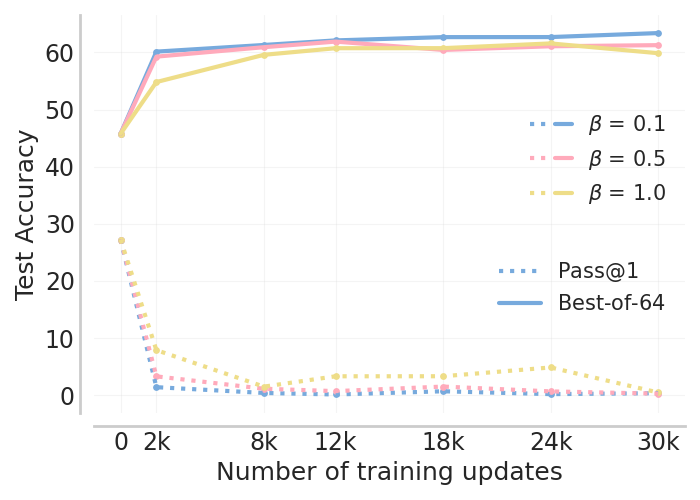
\includegraphics[scale=0.39]{icml2023/figs/ver_vs_gen_colm.png}
  % \caption{Comparing DPO-based generator and verifier for \vstar{} 7B, measured by Pass$@1$ and Verifier$@64$ respectively on GSM8K. Verifier$@64$ accuracy rises significantly while the generation ability of DPO verifier degrades with only 2k training steps.}
    
\end{subfigure}%
\caption{\textbf{Left:} \textbf{Best-of-k test accuracy} of 7B V-STaR compared to \vstar{}[1 Iter] and self-consistency~\citep{DBLP:conf/iclr/0002WSLCNCZ23} across different numbers of candidate solutions generated on GSM8K. We subsample  solutions from $N=1000$ generations. V-STaR can rank over a reasonably large number of candidate solutions. We compute 95\% CIs for self-consistency using 256 trials. \textbf{Right: Comparing DPO-based generator and verifier} for \vstar{} 7B, measured by Pass$@1$ and Best-of-$64$ respectively on GSM8K. Best-of-$64$ accuracy rises significantly while the generation ability of DPO verifier degrades with only 2k updates.}
% \label{fig:ver_at_k}
% \vskip 0.2in

\label{fig:ver_vs_maj}
\label{fig:ver_as_gen}
\end{figure*}
While we use LoRA adapters due to compute constraints,  we hypothesize that gains from \vstar{} could potentially be larger with full parameter fine-tuning.



\textbf{Best-of-$k$ accuracy}. \autoref{fig:ver_at_k} shows test accuracy for $k=1$ to $k=64$, calculated from 128 candidate solutions per test problem, for 7B models on both tasks. Best-of-1 is equivalent to Pass$@1$ and ignores verifier scores. Best-of-$k$ saturates for $k\geq16$ and the gap between \vstar{}~[1 Iter] and \vstar{} stays consistent. 




% Although majority voting is a strong baseline, it cannot be used in tasks such as coding where there is no final answer to be used for voting. 

% \vspace{-0.1cm}

\subsection{Comparing DPO \emph{vs.} ORM verifiers }
\label{sec:dpo}
% \vspace{-0.01in}
We trained ORM style verifiers, as described in \autoref{sec:orm}, with LoRA adapters.
These verifiers did seem to achieve relatively poor performance compared to DPO-based verifiers. \autoref{fig:gsm8k_ver_at_k} shows the comparison between the \vstar{}~[1 Iter] trained with DPO and an ORM style verifier on the same training data. ORM fails to effectively search through generated candidate solutions for number of candidates above 4 in the GSM8K task. The ORM style verifier is also performing worse than our DPO based verifier in MBPP for number of candidate solutions above 16.


% \vspace{-0.25cm}
\subsection{How many completions can V-STaR be extended to?}
\autoref{fig:ver_vs_maj} shows the Best-of-K accuracy of \vstar{}~7B on GSM8K, measured by \autoref{eq:ver_at_k} as a function of $k$. 
\vstar{} outperforms majority voting~\citep{DBLP:conf/iclr/0002WSLCNCZ23} at searching over a large number of candidate solutions (see \autoref{app:vstar_vs_maj_example} in appendix). While \vstar{} is far more effective than majority voting for $k\leq64$, the performance gap starts to slightly decrease for larger value of $k$, similar to performance decay reported in \citet{DBLP:journals/corr/abs-2110-14168}. Furthermore, \vstar{} can be used for any problem solving task where we can verify correctness while majority voting is \textbf{not} applicable to tasks such as code generation. We also tried combining verifier scores with reranking strategies, such as weighted reranking and weighted majority voting \cite{DBLP:journals/corr/abs-2310-10047}, but did not observe performance gains.
% \vspace{-0.03in}

% \vspace{-0.023in}
\subsection{Evaluating DPO verifier as a generator}
\label{sec:dpo_ver_vs_gen}
Since DPO fine-tuned models can also be used as generators, we evaluate how good is the generation ability of DPO verifiers. \autoref{fig:ver_as_gen} shows Pass$@1$ and Best-of-$64$ for V-STaR verifier over training updates, for three different $\beta$ coefficients for proximity to SFT policy in DPO objective~(\autoref{sec:dpo_verifier}). The verifier's solving ability starts degrading only after a small number of training updates. In contrast, using the DPO objective for verification seems to be sample efficient as the model's Best-of-$64$ increases significantly with only $2k$ training updates.

\subsection{Should the verifier be in the training 
loop?}
% \vspace{-0.1cm}
Optionally, one could train intermediate verifiers at each iteration and filter correct solutions to include in $\mathcal{D_\text{GEN}}$ and $\mathcal{D_\text{VER}}$ to provide feedback. This step seems more reasonable with sufficient exploration, that is larger values of $k$, when sampling $k$ solutions from the generator in each iteration.

We tried putting the verifier in the training loop to filter correct solutions from the generator for the next training iteration. To do so, we sampled $k=64$ completions per query from the generator, labeled their correctness, and took only the top 8 based on their verifier score. We take as many samples from the incorrect set so that the total number of correct and incorrect completions per query is 16 or less. 
After running three iterations with verifier in the loop for MBPP, the final Best-of-$64$ accuracy and Pass$@1$ are 53.2 and 46.34 respectively. 

\begin{wrapfigure}{r}{0.5\textwidth}
\vspace*{-1em}
    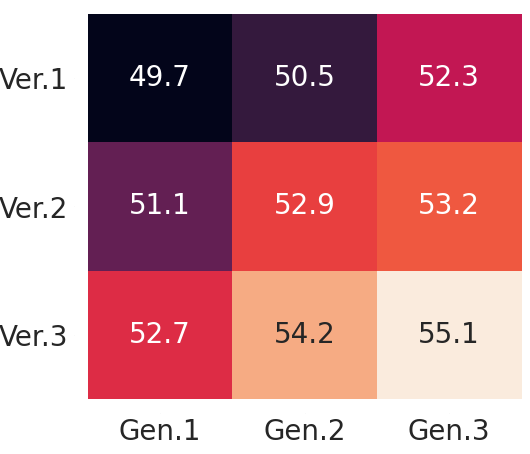
\includegraphics[scale=0.4]{icml2023/figs/mbpp-ver-gen-heatmap-trimmed.png}
\caption{Best-of-64 for each \vstar{} iteration on MBPP. The performance gets better with each iteration of generator and verifier without showing signs of collapsing.}
\label{fig:mbpp_heatmap}
\vspace*{-0.2em}
\end{wrapfigure}

Our results suggest that having the verifier in the training loop does not provide a substantial gain for this task. \vstar{} is simpler without the verifier in the loop and there is no need to train a verifier at each iteration; however we did not experiment with other tasks and different sampling strategies from the generator at each iteration. We leave a more detailed study of this question to future work. 


\subsection{Gains across \vstar{} iteration}
\autoref{fig:mbpp_heatmap} shows the improvements achieved from each iteration of the generator and verifier on MBPP. The gains are larger across iterations of verifiers (from Ver.1 to Ver.3) than iterations of generators which highlights the importance of verifiers. 
% \begin{wrapfigure}[h]
% % \centering
%   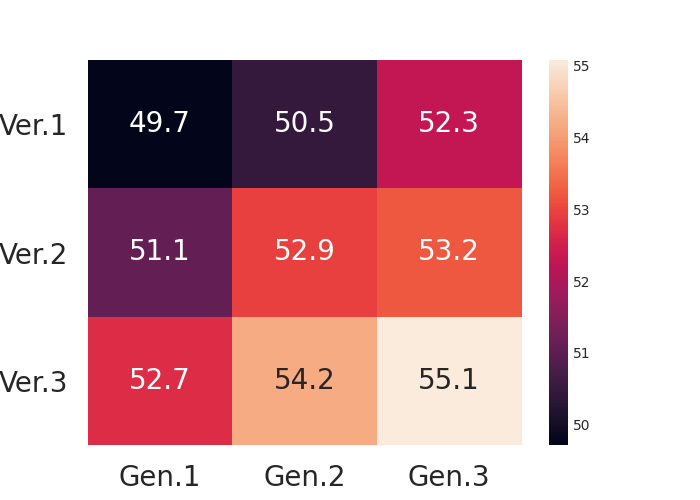
\includegraphics[scale=0.45]{icml2023/figs/mbpp-ver-gen-heatmap.png}
% \caption{Best-of-64 for each \vstar{} iteration on MBPP. The performance gets better with each iteration of generator and verifier without showing signs of collapsing.}
% \label{fig:mbpp_heatmap}
% \end{wrapfigure}


